\section{SR1}
\label{sec:qn-sr1}

BFGS为了保持正定，把负曲率的测量拒之门外。可是目标在某些方向确实向下弯时，这恰恰是有用的信息。这就需要回答：只用一个秩一项能否满足割线条件，这样得到的矩阵有什么长处，又有什么风险？

\paragraph{主要思想：只有一种秩一修正}
设$\bm{B}^{+}=\bm{B}+\sigma\bm{v}\bm{v}^\top$，其中$\sigma=\pm1$。记割线残差$\bm{r}=\bm{y}-\bm{B}\bm{s}$，把割线条件写成
\[
 \sigma\langle\bm{v},\bm{s}\rangle\bm{v}=\bm{r}.
\]
左边是$\bm{v}$的数乘，所以$\bm{v}$必须平行于$\bm{r}$。把$\bm{v}$取成$\bm{r}$的倍数后，$\sigma$和倍数只有一种可能，由此得到\term{对称秩一更新}（symmetric rank-one update，SR1）：
\begin{equation}
 \bm{B}^{+}=\bm{B}+\frac{\bm{r}\bm{r}^\top}{\langle\bm{r},\bm{s}\rangle},\qquad\bm{r}=\bm{y}-\bm{B}\bm{s}.
 \label{eq:qn-sr1-direct}
\end{equation}

与第~\ref{sec:qn-dfp-bfgs}节不同，这里的更新由割线条件和“秩一”完全确定，没有选择余地。验算割线条件：$\bm{B}^{+}\bm{s}=\bm{B}\bm{s}+\bm{r}=\bm{y}$。

把同样的推导用在逆矩阵上，并记$\bm{w}=\bm{s}-\bm{W}\bm{y}$，得到
\begin{equation}
 \bm{W}^{+}=\bm{W}+\frac{\bm{w}\bm{w}^\top}{\langle\bm{w},\bm{y}\rangle}.
 \label{eq:qn-sr1-inverse}
\end{equation}
只要$\bm{B}$、$\bm{B}^{+}$都可逆，式~\eqref{eq:qn-sr1-inverse}的$\bm{W}^{+}$就是式~\eqref{eq:qn-sr1-direct}的$\bm{B}^{+}$的逆，这可以用Sherman--Morrison公式验证。SR1自己是自己的对偶，所以不像BFGS和DFP那样分成两种方法。

\paragraph{计算过程}
SR1不需要线搜索来保持什么性质，下面就用单位步长演示它。仍用贯穿例，这一次不做线搜索，每步直接走完整的$-\bm{W}^{(t)}\bm{g}^{(t)}$。

\needspace{6\baselineskip}
\paragraph{变量}
\begin{itemize}
 \item $\bm{x}^{(t)}$、$\bm{g}^{(t)}\in\mathbb{R}^{n}$：当前点与梯度。
 \item $\bm{W}^{(t)}\in\mathbb{R}^{n\times n}$：对称的逆曲率近似，不要求正定。
 \item $\bm{s}^{(t)}$、$\bm{y}^{(t)}$：位移与梯度差；$\bm{w}^{(t)}$：式~\eqref{eq:qn-sr1-inverse}中逆形式的割线残差。
 \item $c_{\mathrm{r}}>0$：判断分母是否过小的阈值。
\end{itemize}

\paragraph{初始化}
选起点和对称的$\bm{W}^{(0)}$。例中初始数据是
\[
 \bm{x}^{(0)}=(4,1)^\top,\qquad\bm{W}^{(0)}=\bm{I},\qquad\bm{g}^{(0)}=(8,8)^\top.
\]

\paragraph{每轮更新}
对$t=0,1,\ldots$依次执行下面的步骤，当$\lVert\bm{g}^{(t)}\rVert_2\leq\varepsilon$时停止。

\begin{enumerate}
\item 计算$\bm{s}^{(t)}=-\bm{W}^{(t)}\bm{g}^{(t)}$，令$\bm{x}^{(t+1)}=\bm{x}^{(t)}+\bm{s}^{(t)}$，并读取$\bm{g}^{(t+1)}$。例中第一轮得到
\[
 \bm{s}^{(0)}=(-8,-8)^\top,\qquad\bm{x}^{(1)}=(-4,-7)^\top,\qquad\bm{g}^{(1)}=(-8,-56)^\top.
\]
目标值从$20$升到了$212$，这一步在目标上是失败的，但测量仍然有用。

\item 计算$\bm{y}^{(t)}=\bm{g}^{(t+1)}-\bm{g}^{(t)}$和$\bm{w}^{(t)}$。例中第一轮得到
\[
 \bm{y}^{(0)}=(-16,-64)^\top,\qquad\bm{w}^{(0)}=(8,56)^\top,\qquad\langle\bm{w}^{(0)},\bm{y}^{(0)}\rangle=-3712.
\]

\item 若$\langle\bm{w}^{(t)},\bm{y}^{(t)}\rangle$的绝对值不小于$c_{\mathrm{r}}\lVert\bm{w}^{(t)}\rVert_2\lVert\bm{y}^{(t)}\rVert_2$，由式~\eqref{eq:qn-sr1-inverse}更新$\bm{W}^{(t+1)}$；否则令$\bm{W}^{(t+1)}=\bm{W}^{(t)}$。例中第一轮分母足够大，更新后得到
\[
 \bm{W}^{(1)}=\frac{1}{58}\begin{bmatrix}57&-7\\-7&9\end{bmatrix}.
\]
\end{enumerate}

第二轮的位移与新点是
\[
 \bm{s}^{(1)}=\frac{1}{29}(32,224)^\top,\qquad\bm{x}^{(2)}=\frac{1}{29}(-84,21)^\top\approx(-2.897,0.724)^\top.
\]

梯度差和逆形式残差是
\[
 \bm{y}^{(1)}=\frac{1}{29}(64,1792)^\top,\qquad\bm{w}^{(1)}=\frac{1344}{841}(4,-1)^\top.
\]

分母约为$-84.64$，更新量是$-\tfrac{7}{232}$乘以$\begin{bmatrix}16&-4\\-4&1\end{bmatrix}$，于是
\[
 \bm{W}^{(2)}=\begin{bmatrix}0.5&0\\0&0.125\end{bmatrix}=\bm{A}^{-1}.
\]

第三轮的方向已经是Newton方向，一步到达解：
\[
 \bm{s}^{(2)}=\frac{1}{29}(84,-21)^\top,\qquad\bm{x}^{(3)}=\bm{0},\qquad\bm{g}^{(3)}=\bm{0}.
\]
迭代结束，最终得到解$\bm{x}^{(3)}=\bm{0}$，用了$n+1=3$步。图~\ref{fig:qn-sr1-path}是这条路径。

\begin{BookInlineFigure}
  \centering
  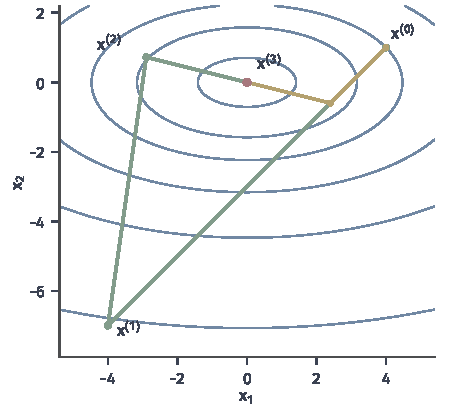
\includegraphics[width=78mm]{figures/05-optimization/02-smooth-optimization/matplotlib/qn-sr1-path/figure.pdf}
  \caption{贯穿例上的SR1路径（绿）：$\bm{W}^{(0)}=\bm{I}$，每步取单位步长。第一步远远越过谷底，目标值从$20$升到$212$，但两次测量足以确定$\bm{A}$，第三步准确落在最优解（红）。黄线是精确线搜索的BFGS路径，用作对照。}
  \label{fig:qn-sr1-path}
\end{BookInlineFigure}

\paragraph{有限步终止}
这个现象对二次目标普遍成立，而且完全不依赖步长的选取。下面的定理把BFGS那里“两次测量都不丢失”的现象，以更强的形式写了下来。

\begin{theorem}[SR1的遗传性质]
\label{thm:qn-sr1-hereditary}
设$f$是二次函数，Hessian为对称矩阵$\bm{A}$，于是$\bm{y}^{(j)}=\bm{A}\bm{s}^{(j)}$。设$\bm{B}^{(j+1)}$由SR1按式~\eqref{eq:qn-sr1-direct}逐次得到，所有分母非零。则对每个$k$，
\begin{equation}
 \bm{B}^{(k)}\bm{s}^{(j)}=\bm{y}^{(j)},\qquad j=0,1,\ldots,k-1.
 \label{eq:qn-sr1-hereditary}
\end{equation}
特别地，若$\bm{s}^{(0)},\ldots,\bm{s}^{(n-1)}$线性无关，则$\bm{B}^{(n)}=\bm{A}$。
\end{theorem}

\begin{proof}
对$k$归纳。$k=1$时就是割线条件。设式~\eqref{eq:qn-sr1-hereditary}对$k$成立，并记$\bm{r}=\bm{y}^{(k)}-\bm{B}^{(k)}\bm{s}^{(k)}$。

对$j<k$，由归纳假设、对称性和$\bm{y}^{(j)}=\bm{A}\bm{s}^{(j)}$，得到
\[
 \begin{aligned}
 \langle\bm{r},\bm{s}^{(j)}\rangle
 &=\langle\bm{y}^{(k)},\bm{s}^{(j)}\rangle-\langle\bm{s}^{(k)},\bm{B}^{(k)}\bm{s}^{(j)}\rangle\\
 &=\langle\bm{A}\bm{s}^{(k)},\bm{s}^{(j)}\rangle-\langle\bm{s}^{(k)},\bm{A}\bm{s}^{(j)}\rangle=0.
 \end{aligned}
\]

所以秩一修正项作用在旧位移上为零：
\[
 \bm{B}^{(k+1)}\bm{s}^{(j)}=\bm{B}^{(k)}\bm{s}^{(j)}+\bm{r}\,\frac{\langle\bm{r},\bm{s}^{(j)}\rangle}{\langle\bm{r},\bm{s}^{(k)}\rangle}=\bm{y}^{(j)}.
\]
$j=k$时是割线条件本身，归纳完成。

$\bm{s}^{(j)}$线性无关时，把它们排成可逆矩阵$\bm{S}$，式~\eqref{eq:qn-sr1-hereditary}说明$\bm{B}^{(n)}\bm{S}=\bm{A}\bm{S}$，右乘$\bm{S}^{-1}$即得。
\end{proof}

所以$\bm{A}$可逆、$\bm{B}^{(n)}$之前的各步线性无关时，单位步长的SR1至多$n+1$步到达驻点。定理没有要求$\bm{A}$正定，也没有要求线搜索，这是SR1与BFGS的重要区别。

\paragraph{分母可能为零}
SR1的麻烦全在分母$\langle\bm{r},\bm{s}\rangle$上。若$\bm{r}\neq\bm{0}$而$\langle\bm{r},\bm{s}\rangle=0$，则根本不存在满足割线条件的对称秩一修正。原因是由$\sigma\langle\bm{v},\bm{s}\rangle\bm{v}=\bm{r}$与$\bm{s}$作内积，得到
\[
 \sigma\langle\bm{v},\bm{s}\rangle^2=\langle\bm{r},\bm{s}\rangle=0.
\]
于是$\langle\bm{v},\bm{s}\rangle=0$，等式左边就是零向量，与$\bm{r}\neq\bm{0}$矛盾。

这种情况确实会出现。取$\bm{A}=\operatorname{diag}(2,8)$，$\bm{B}=\operatorname{diag}(3,7)$，$\bm{s}=(1,1)^\top$，则
\[
 \bm{y}=(2,8)^\top,\qquad\bm{r}=(-1,1)^\top,\qquad\langle\bm{r},\bm{s}\rangle=0.
\]

分母接近零同样有害。把$\bm{s}$换成$(1,1+\epsilon)^\top$，分母是$2\epsilon+\epsilon^2$，而$\lVert\bm{r}\rVert_2$约为$\sqrt2$，修正量的Frobenius范数约为$1/\epsilon$。图~\ref{fig:qn-sr1-denominator}展示了这种放大：$\epsilon=10^{-4}$时修正量约为$10^{4}$，矩阵几乎被这一次修正淹没。

\begin{BookInlineFigure}
  \centering
  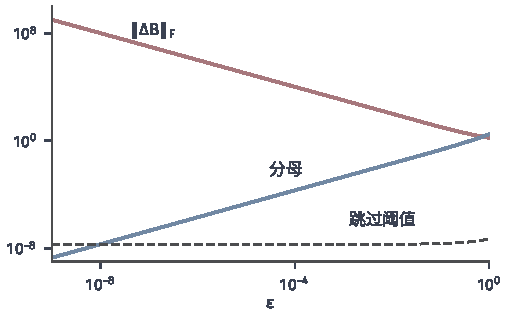
\includegraphics[width=86mm]{figures/05-optimization/02-smooth-optimization/matplotlib/qn-sr1-denominator/figure.pdf}
  \caption{SR1的分母接近零时的放大效应：$\bm{A}=\operatorname{diag}(2,8)$，$\bm{B}=\operatorname{diag}(3,7)$，$\bm{s}=(1,1+\epsilon)^\top$。蓝线是分母$\lvert\langle\bm{r},\bm{s}\rangle\rvert$，红线是修正量$\lVert\Delta\bm{B}\rVert_F$；虚线是取$c_{\mathrm{r}}=10^{-8}$时的跳过阈值$c_{\mathrm{r}}\lVert\bm{r}\rVert_2\lVert\bm{s}\rVert_2$，分母低于它就不更新。}
  \label{fig:qn-sr1-denominator}
\end{BookInlineFigure}

所以SR1配有跳过规则，这就是计算过程第三步的判断，直接形式下写成
\begin{equation}
 \lvert\langle\bm{r},\bm{s}\rangle\rvert\geq c_{\mathrm{r}}\lVert\bm{r}\rVert_2\lVert\bm{s}\rVert_2,
 \label{eq:qn-sr1-safeguard}
\end{equation}
通常取$c_{\mathrm{r}}=10^{-8}$。不满足时保持$\bm{B}^{+}=\bm{B}$。

式~\eqref{eq:qn-sr1-safeguard}中的角度形式比绝对阈值合理：它问的是$\bm{r}$与$\bm{s}$是否几乎垂直，与两个向量的长度无关。跳过很少发生，因为分母近零需要$\bm{r}$恰好几乎垂直于$\bm{s}$。

\paragraph{SR1通常不保持正定}
BFGS的更新中，分母$\langle\bm{s},\bm{y}\rangle$与修正项的符号都受控制。SR1的分母可正可负，修正项的符号跟着变，所以正定矩阵可能变成不定矩阵，即使目标强凸。

取贯穿例的目标，$\bm{x}^{(0)}=(-4,-0.5)^\top$，$\bm{B}^{(0)}=4\bm{I}$，单位步长。这时
\[
 \bm{g}^{(0)}=(-8,-4)^\top,\qquad\bm{s}^{(0)}=(2,1)^\top,\qquad\bm{y}^{(0)}=(4,8)^\top.
\]

$\bm{B}^{(0)}\bm{s}^{(0)}=(8,4)^\top$，所以残差和分母是
\[
 \bm{r}=(-4,4)^\top,\qquad\langle\bm{r},\bm{s}^{(0)}\rangle=-4.
\]
代入式~\eqref{eq:qn-sr1-direct}，得到
\[
 \bm{B}^{(1)}=\begin{bmatrix}0&4\\4&0\end{bmatrix}.
\]
它的特征值是$\pm4$，不定。验算割线条件：$\bm{B}^{(1)}\bm{s}^{(0)}=(4,8)^\top=\bm{y}^{(0)}$。

新点是$\bm{x}^{(1)}=(-2,0.5)^\top$，梯度$\bm{g}^{(1)}=(-4,4)^\top$。若仍然用公式~\eqref{eq:qn-direction}算方向，得到
\[
 \bm{d}=-\bigl(\bm{B}^{(1)}\bigr)^{-1}\bm{g}^{(1)}=(-1,1)^\top,\qquad\langle\bm{g}^{(1)},\bm{d}\rangle=8>0.
\]

这是一个上升方向。$\bm{d}$是模型的驻点，但模型不定，驻点是鞍点而不是极小点。沿它走一步，目标从$5$升到$18$。第~\ref{sec:qn-secant}节的下降论证依赖$\bm{W}$正定，这里前提已经不成立，所以不能把BFGS方向的下降分析搬过来。

\paragraph{不定模型与信赖域}
不定的$\bm{B}$并非无用，用错的只是“跑到模型驻点”这个做法。模型$m(\bm{p})$在$\bm{p}$的某些方向向下弯，这时它没有极小点，但在一个有界的范围内它有。第~\ref{chap:trust-region}章的信赖域方法正是如此：只在以当前点为中心、半径为$\Delta$的球内最小化模型，并用实际下降检验这个候选步。

继续上面的例子，取$\Delta=1$。$\bm{B}^{(1)}$的负特征值$-4$对应单位特征向量$\bm{v}=(1,-1)^\top/\sqrt2$，而$\bm{g}^{(1)}=-4\sqrt2\,\bm{v}$恰好全部落在这个方向上。沿$\bm{p}=\beta\bm{v}$，模型的变化量是
\[
 m(\beta\bm{v})-m(\bm{0})=-4\sqrt2\,\beta-2\beta^2.
\]

在$\lvert\beta\rvert\leq1$上它在$\beta=1$处最小，所以候选步是
\[
 \bm{p}_{\Delta}=\frac{1}{\sqrt2}(1,-1)^\top.
\]
它是下降方向，因为与梯度的内积是$-4\sqrt2<0$。沿它走一步，目标从$5$降到约$1.843$。图~\ref{fig:qn-sr1-saddle}比较了两个候选步。

\begin{BookInlineFigure}
  \centering
  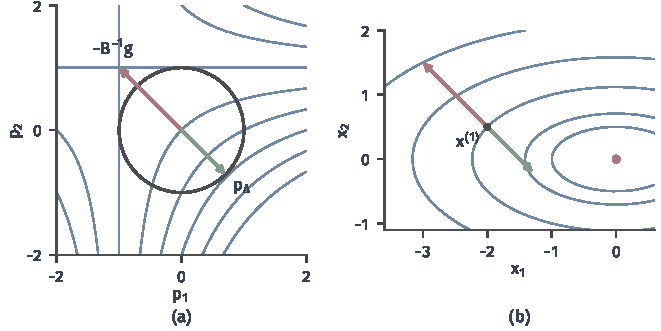
\includegraphics[width=112mm]{figures/05-optimization/02-smooth-optimization/matplotlib/qn-sr1-saddle/figure.pdf}
  \caption{不定模型下的两个候选步，$\bm{B}=\begin{bmatrix}0&4\\4&0\end{bmatrix}$，$\bm{g}=(-4,4)^\top$，圆的半径为$1$。(a)蓝线是模型$m(\bm{p})$的等值线，呈鞍形。红箭头是模型的驻点$-\bm{B}^{-1}\bm{g}$，绿箭头是圆内模型的极小点。(b)同样的两步放到真实目标$x_1^2+4x_2^2$的等高线上，红步使目标上升，绿步使目标下降。}
  \label{fig:qn-sr1-saddle}
\end{BookInlineFigure}

这也解释了SR1和BFGS的分工。BFGS的矩阵总是正定的，方向一定下降，配线搜索很自然；但它看不到负曲率，也只有测量满足曲率条件才能更新。SR1能记录负曲率，在二次目标上对步长没有要求，但需要有界的模型来消化不定性。

\begin{BookInlineTable}
  \centering
  \begin{tabular}{lll}
    \toprule
    比较项 & BFGS & SR1\\
    \midrule
    修正的秩 & 二 & 一\\
    更新的前提 & 曲率条件 & 分母不过小\\
    正定性 & 保持 & 通常不保持\\
    负曲率信息 & 不能表示 & 可以表示\\
    配套的全局化手段 & Wolfe线搜索 & 信赖域\\
    \bottomrule
  \end{tabular}
  \caption{BFGS与SR1的对比。}
  \label{tab:qn-bfgs-sr1}
\end{BookInlineTable}
